%----------------------------------------------------------------------------------------
%	PACKAGES AND OTHER DOCUMENT CONFIGURATIONS
%----------------------------------------------------------------------------------------
\documentclass[a4paper,11pt]{article}
\usepackage[a4paper,textwidth=140mm,textheight=245mm]{geometry}
\usepackage[utf8]{inputenc}
\usepackage{listings}
\usepackage{graphicx}
\usepackage{pstricks}
\usepackage{tikz}
\usepackage{float}
\makeatletter
\renewcommand{\section}{\@startsection
   {section}%                         name
   {1}%                               level
   {0mm}%                             indent
   {-1.5\baselineskip}%               space above header
   {0.5\baselineskip}%                space under header
   {\sffamily\bfseries\upshape\normalsize}}% style
   
\renewcommand{\subsection}{\@startsection
   {subsection}%                      name
   {2}%                               level
   {0mm}%                             indent
   {-0.75\baselineskip}%              space above header
   {0.25\baselineskip}%               space under header
   {\rmfamily\normalfont\slshape\normalsize}}% style
\renewcommand{\subsubsection}{\@startsection
   {subsubsection}%                    name
   {3}%                               level
   {0mm}%                             indent
   {-0.75\baselineskip}%              space above header
   {0.25\baselineskip}%               space under header
   {\rmfamily\normalfont\slshape\normalsize}}% style
\makeatother
\begin{document}
\begin{titlepage}
\title{TDDB68 sammanfattning}
\author{Martin Söderén\\ marso329@student.liu.se\\900929-1098}
\date{\today}
\maketitle




\vfill % Fill the rest of the page with whitespace

\thispagestyle{empty}

\end{titlepage}
\section{Processer och trådar}
\subsection{schemaläggning}
\begin{figure}[h]
\scalebox{0.8}{% Graphic for TeX using PGF
% Title: /home/martin/tddb68/process_state.dia
% Creator: Dia v0.97.2
% CreationDate: Thu Mar 12 14:28:46 2015
% For: martin
% \usepackage{tikz}
% The following commands are not supported in PSTricks at present
% We define them conditionally, so when they are implemented,
% this pgf file will use them.
\ifx\du\undefined
  \newlength{\du}
\fi
\setlength{\du}{15\unitlength}
\begin{tikzpicture}
\pgftransformxscale{1.000000}
\pgftransformyscale{-1.000000}
\definecolor{dialinecolor}{rgb}{0.000000, 0.000000, 0.000000}
\pgfsetstrokecolor{dialinecolor}
\definecolor{dialinecolor}{rgb}{1.000000, 1.000000, 1.000000}
\pgfsetfillcolor{dialinecolor}
\pgfsetlinewidth{0.100000\du}
\pgfsetdash{}{0pt}
{\pgfsetcornersarced{\pgfpoint{0.500000\du}{0.500000\du}}\definecolor{dialinecolor}{rgb}{1.000000, 1.000000, 1.000000}
\pgfsetfillcolor{dialinecolor}
\fill (1.200000\du,1.200000\du)--(1.200000\du,3.000000\du)--(5.200000\du,3.000000\du)--(5.200000\du,1.200000\du)--cycle;
}{\pgfsetcornersarced{\pgfpoint{0.500000\du}{0.500000\du}}\definecolor{dialinecolor}{rgb}{0.000000, 0.000000, 0.000000}
\pgfsetstrokecolor{dialinecolor}
\draw (1.200000\du,1.200000\du)--(1.200000\du,3.000000\du)--(5.200000\du,3.000000\du)--(5.200000\du,1.200000\du)--cycle;
}% setfont left to latex
\definecolor{dialinecolor}{rgb}{0.000000, 0.000000, 0.000000}
\pgfsetstrokecolor{dialinecolor}
\node at (3.200000\du,2.295000\du){new};
\pgfsetlinewidth{0.100000\du}
\pgfsetdash{}{0pt}
{\pgfsetcornersarced{\pgfpoint{0.500000\du}{0.500000\du}}\definecolor{dialinecolor}{rgb}{1.000000, 1.000000, 1.000000}
\pgfsetfillcolor{dialinecolor}
\fill (8.162891\du,4.250000\du)--(8.162891\du,6.050000\du)--(12.162891\du,6.050000\du)--(12.162891\du,4.250000\du)--cycle;
}{\pgfsetcornersarced{\pgfpoint{0.500000\du}{0.500000\du}}\definecolor{dialinecolor}{rgb}{0.000000, 0.000000, 0.000000}
\pgfsetstrokecolor{dialinecolor}
\draw (8.162891\du,4.250000\du)--(8.162891\du,6.050000\du)--(12.162891\du,6.050000\du)--(12.162891\du,4.250000\du)--cycle;
}% setfont left to latex
\definecolor{dialinecolor}{rgb}{0.000000, 0.000000, 0.000000}
\pgfsetstrokecolor{dialinecolor}
\node at (10.162891\du,5.345000\du){ready};
\pgfsetlinewidth{0.100000\du}
\pgfsetdash{}{0pt}
\pgfsetdash{}{0pt}
\pgfsetbuttcap
{
\definecolor{dialinecolor}{rgb}{0.000000, 0.000000, 0.000000}
\pgfsetfillcolor{dialinecolor}
% was here!!!
\pgfsetarrowsend{latex}
\definecolor{dialinecolor}{rgb}{0.000000, 0.000000, 0.000000}
\pgfsetstrokecolor{dialinecolor}
\draw (5.248409\du,2.997278\du)--(8.114482\du,4.252722\du);
}
\pgfsetlinewidth{0.100000\du}
\pgfsetdash{}{0pt}
{\pgfsetcornersarced{\pgfpoint{0.500000\du}{0.500000\du}}\definecolor{dialinecolor}{rgb}{1.000000, 1.000000, 1.000000}
\pgfsetfillcolor{dialinecolor}
\fill (19.200000\du,4.250000\du)--(19.200000\du,6.050000\du)--(23.200000\du,6.050000\du)--(23.200000\du,4.250000\du)--cycle;
}{\pgfsetcornersarced{\pgfpoint{0.500000\du}{0.500000\du}}\definecolor{dialinecolor}{rgb}{0.000000, 0.000000, 0.000000}
\pgfsetstrokecolor{dialinecolor}
\draw (19.200000\du,4.250000\du)--(19.200000\du,6.050000\du)--(23.200000\du,6.050000\du)--(23.200000\du,4.250000\du)--cycle;
}% setfont left to latex
\definecolor{dialinecolor}{rgb}{0.000000, 0.000000, 0.000000}
\pgfsetstrokecolor{dialinecolor}
\node at (21.200000\du,5.345000\du){running};
\pgfsetlinewidth{0.100000\du}
\pgfsetdash{}{0pt}
{\pgfsetcornersarced{\pgfpoint{0.500000\du}{0.500000\du}}\definecolor{dialinecolor}{rgb}{1.000000, 1.000000, 1.000000}
\pgfsetfillcolor{dialinecolor}
\fill (26.200000\du,1.200000\du)--(26.200000\du,3.000000\du)--(30.747500\du,3.000000\du)--(30.747500\du,1.200000\du)--cycle;
}{\pgfsetcornersarced{\pgfpoint{0.500000\du}{0.500000\du}}\definecolor{dialinecolor}{rgb}{0.000000, 0.000000, 0.000000}
\pgfsetstrokecolor{dialinecolor}
\draw (26.200000\du,1.200000\du)--(26.200000\du,3.000000\du)--(30.747500\du,3.000000\du)--(30.747500\du,1.200000\du)--cycle;
}% setfont left to latex
\definecolor{dialinecolor}{rgb}{0.000000, 0.000000, 0.000000}
\pgfsetstrokecolor{dialinecolor}
\node at (28.473750\du,2.295000\du){terminated};
\pgfsetlinewidth{0.100000\du}
\pgfsetdash{}{0pt}
\pgfsetdash{}{0pt}
\pgfsetbuttcap
{
\definecolor{dialinecolor}{rgb}{0.000000, 0.000000, 0.000000}
\pgfsetfillcolor{dialinecolor}
% was here!!!
\pgfsetarrowsend{latex}
\definecolor{dialinecolor}{rgb}{0.000000, 0.000000, 0.000000}
\pgfsetstrokecolor{dialinecolor}
\draw (23.249738\du,4.290512\du)--(26.211358\du,3.048657\du);
}
\pgfsetlinewidth{0.100000\du}
\pgfsetdash{}{0pt}
{\pgfsetcornersarced{\pgfpoint{0.500000\du}{0.500000\du}}\definecolor{dialinecolor}{rgb}{1.000000, 1.000000, 1.000000}
\pgfsetfillcolor{dialinecolor}
\fill (14.200000\du,8.200000\du)--(14.200000\du,10.000000\du)--(18.200000\du,10.000000\du)--(18.200000\du,8.200000\du)--cycle;
}{\pgfsetcornersarced{\pgfpoint{0.500000\du}{0.500000\du}}\definecolor{dialinecolor}{rgb}{0.000000, 0.000000, 0.000000}
\pgfsetstrokecolor{dialinecolor}
\draw (14.200000\du,8.200000\du)--(14.200000\du,10.000000\du)--(18.200000\du,10.000000\du)--(18.200000\du,8.200000\du)--cycle;
}% setfont left to latex
\definecolor{dialinecolor}{rgb}{0.000000, 0.000000, 0.000000}
\pgfsetstrokecolor{dialinecolor}
\node at (16.200000\du,9.295000\du){waiting};
\pgfsetlinewidth{0.100000\du}
\pgfsetdash{}{0pt}
\pgfsetdash{}{0pt}
\pgfsetbuttcap
{
\definecolor{dialinecolor}{rgb}{0.000000, 0.000000, 0.000000}
\pgfsetfillcolor{dialinecolor}
% was here!!!
\pgfsetarrowsend{latex}
\definecolor{dialinecolor}{rgb}{0.000000, 0.000000, 0.000000}
\pgfsetstrokecolor{dialinecolor}
\draw (19.997607\du,6.099890\du)--(17.402393\du,8.150110\du);
}
\pgfsetlinewidth{0.100000\du}
\pgfsetdash{}{0pt}
\pgfsetdash{}{0pt}
\pgfsetbuttcap
{
\definecolor{dialinecolor}{rgb}{0.000000, 0.000000, 0.000000}
\pgfsetfillcolor{dialinecolor}
% was here!!!
\pgfsetarrowsend{latex}
\definecolor{dialinecolor}{rgb}{0.000000, 0.000000, 0.000000}
\pgfsetstrokecolor{dialinecolor}
\draw (14.748205\du,8.150110\du)--(11.614686\du,6.099890\du);
}
\pgfsetlinewidth{0.100000\du}
\pgfsetdash{}{0pt}
\pgfsetdash{}{0pt}
\pgfsetbuttcap
{
\definecolor{dialinecolor}{rgb}{0.000000, 0.000000, 0.000000}
\pgfsetfillcolor{dialinecolor}
% was here!!!
\pgfsetarrowsend{latex}
\definecolor{dialinecolor}{rgb}{0.000000, 0.000000, 0.000000}
\pgfsetstrokecolor{dialinecolor}
\pgfpathmoveto{\pgfpoint{20.407398\du}{4.200436\du}}
\pgfpatharc{315}{226}{6.700767\du and 6.700767\du}
\pgfusepath{stroke}
}
\pgfsetlinewidth{0.100000\du}
\pgfsetdash{}{0pt}
\pgfsetdash{}{0pt}
\pgfsetbuttcap
{
\definecolor{dialinecolor}{rgb}{0.000000, 0.000000, 0.000000}
\pgfsetfillcolor{dialinecolor}
% was here!!!
\pgfsetarrowsend{latex}
\definecolor{dialinecolor}{rgb}{0.000000, 0.000000, 0.000000}
\pgfsetstrokecolor{dialinecolor}
\draw (12.212139\du,5.150000\du)--(19.150752\du,5.150000\du);
}
% setfont left to latex
\definecolor{dialinecolor}{rgb}{0.000000, 0.000000, 0.000000}
\pgfsetstrokecolor{dialinecolor}
\node[anchor=west] at (6.400000\du,2.800000\du){admitted};
% setfont left to latex
\definecolor{dialinecolor}{rgb}{0.000000, 0.000000, 0.000000}
\pgfsetstrokecolor{dialinecolor}
\node[anchor=west] at (14.600000\du,1.750000\du){interrupt};
% setfont left to latex
\definecolor{dialinecolor}{rgb}{0.000000, 0.000000, 0.000000}
\pgfsetstrokecolor{dialinecolor}
\node[anchor=west] at (23.750000\du,3.300000\du){exit};
% setfont left to latex
\definecolor{dialinecolor}{rgb}{0.000000, 0.000000, 0.000000}
\pgfsetstrokecolor{dialinecolor}
\node[anchor=west] at (19.950000\du,7.750000\du){I/O or event wait};
% setfont left to latex
\definecolor{dialinecolor}{rgb}{0.000000, 0.000000, 0.000000}
\pgfsetstrokecolor{dialinecolor}
\node[anchor=west] at (5.600000\du,7.800000\du){I/O or event completion};
% setfont left to latex
\definecolor{dialinecolor}{rgb}{0.000000, 0.000000, 0.000000}
\pgfsetstrokecolor{dialinecolor}
\node[anchor=west] at (12.700000\du,4.750000\du){scheduler dispatch};
\end{tikzpicture}
}
\caption{diagram av processstadier} 
\end{figure}
\subsection{Multilevel Feedback Queue}
Processer placeras i en kö beroende på prioritet. När en process har körts så ökas alla andras prioritet med ett och processen placeras i kön igen.
\subsection{round-robin}
Processortiden delas in i tidskvoter om t.ex 100ms. En process körs då i 100ms och byts sedan ut oavsett om den är klar eller ej. Kräver preemptive.
\subsection{shortest job first}
Av alla processer som väntar så tas den som förvantas tas kortast tid.
\subsection{FIFO}
Vet du inte vad fifo är så är du körd.
\subsection{preemptive schedular}
Ett operativsystem som stödjer detta har möjligtheten att avbryta en process och låta en annan använda processerna istället. Motsatsen är nonpreemtive och då måste varje process självmant ge upp processorn.
\subsection{process/task control block}
Representerar varje process i operativsystemet. Innehåller bland annat:
\begin{itemize}
\item process state - new,ready ....
\item program counter
\item CPU registers
\item CPU-scheduling information - priority and so on
\item Memory management informaition - basen på stacken bland annat
\item accouting information - hur mycket processen har förbrukat
\item I/O status information - öppna enheter och filer
\end{itemize}
\subsection{processer/trådar}
En process ger resurser för att ett program ska kunna slutföras. Har ett eget adressutrymme och en egen pid. En tråd existerar inom en process och en process kan ha flera trådar. \\ \\
\subsection{many-to-many}
I ett many-to-many system så blockeras inte alla trådar, dock alla i samma process. Det utnyttjar flera processorer. Behöver dock en schemaläggare i userland.
\subsection{one-to-many}
Kan skapa många trådar. Kan inte utnyttja flera cpu:er. I/O operationer kan blockera alla trådar.
\subsection{one-to-one}
Trådar blockerar inte varandra. Trådar kan köras på olika cpu:er. Kan bara skapa en begränsad mång trådar.
\subsection{systemanrop}
\begin{figure}[H]
\scalebox{0.8}{% Graphic for TeX using PGF
% Title: /home/martin/tddb68/latex/user_kernel.dia
% Creator: Dia v0.97.2
% CreationDate: Fri Mar 13 16:46:30 2015
% For: martin
% \usepackage{tikz}
% The following commands are not supported in PSTricks at present
% We define them conditionally, so when they are implemented,
% this pgf file will use them.
\ifx\du\undefined
  \newlength{\du}
\fi
\setlength{\du}{15\unitlength}
\begin{tikzpicture}
\pgftransformxscale{1.000000}
\pgftransformyscale{-1.000000}
\definecolor{dialinecolor}{rgb}{0.000000, 0.000000, 0.000000}
\pgfsetstrokecolor{dialinecolor}
\definecolor{dialinecolor}{rgb}{1.000000, 1.000000, 1.000000}
\pgfsetfillcolor{dialinecolor}
\pgfsetlinewidth{0.100000\du}
\pgfsetdash{}{0pt}
\pgfsetdash{}{0pt}
\pgfsetmiterjoin
\definecolor{dialinecolor}{rgb}{1.000000, 1.000000, 1.000000}
\pgfsetfillcolor{dialinecolor}
\fill (5.000000\du,1.300000\du)--(5.000000\du,7.300000\du)--(30.000000\du,7.300000\du)--(30.000000\du,1.300000\du)--cycle;
\definecolor{dialinecolor}{rgb}{0.000000, 0.000000, 0.000000}
\pgfsetstrokecolor{dialinecolor}
\draw (5.000000\du,1.300000\du)--(5.000000\du,7.300000\du)--(30.000000\du,7.300000\du)--(30.000000\du,1.300000\du)--cycle;
\pgfsetlinewidth{0.100000\du}
\pgfsetdash{}{0pt}
\pgfsetdash{}{0pt}
\pgfsetmiterjoin
\definecolor{dialinecolor}{rgb}{1.000000, 1.000000, 1.000000}
\pgfsetfillcolor{dialinecolor}
\fill (5.000000\du,9.300000\du)--(5.000000\du,15.300000\du)--(30.000000\du,15.300000\du)--(30.000000\du,9.300000\du)--cycle;
\definecolor{dialinecolor}{rgb}{0.000000, 0.000000, 0.000000}
\pgfsetstrokecolor{dialinecolor}
\draw (5.000000\du,9.300000\du)--(5.000000\du,15.300000\du)--(30.000000\du,15.300000\du)--(30.000000\du,9.300000\du)--cycle;
\pgfsetlinewidth{0.100000\du}
\pgfsetdash{}{0pt}
\pgfsetdash{}{0pt}
\pgfsetbuttcap
{
\definecolor{dialinecolor}{rgb}{0.000000, 0.000000, 0.000000}
\pgfsetfillcolor{dialinecolor}
% was here!!!
\definecolor{dialinecolor}{rgb}{0.000000, 0.000000, 0.000000}
\pgfsetstrokecolor{dialinecolor}
\draw (2.000000\du,8.300000\du)--(33.000000\du,8.300000\du);
}
% setfont left to latex
\definecolor{dialinecolor}{rgb}{0.000000, 0.000000, 0.000000}
\pgfsetstrokecolor{dialinecolor}
\node[anchor=west] at (17.500000\du,4.300000\du){};
% setfont left to latex
\definecolor{dialinecolor}{rgb}{0.000000, 0.000000, 0.000000}
\pgfsetstrokecolor{dialinecolor}
\node[anchor=west] at (6.000000\du,2.300000\du){user process};
% setfont left to latex
\definecolor{dialinecolor}{rgb}{0.000000, 0.000000, 0.000000}
\pgfsetstrokecolor{dialinecolor}
\node[anchor=west] at (6.000000\du,10.300000\du){kernel};
\pgfsetlinewidth{0.100000\du}
\pgfsetdash{}{0pt}
\pgfsetdash{}{0pt}
\pgfsetmiterjoin
\definecolor{dialinecolor}{rgb}{1.000000, 1.000000, 1.000000}
\pgfsetfillcolor{dialinecolor}
\fill (6.000000\du,4.300000\du)--(6.000000\du,6.300000\du)--(11.000000\du,6.300000\du)--(11.000000\du,4.300000\du)--cycle;
\definecolor{dialinecolor}{rgb}{0.000000, 0.000000, 0.000000}
\pgfsetstrokecolor{dialinecolor}
\draw (6.000000\du,4.300000\du)--(6.000000\du,6.300000\du)--(11.000000\du,6.300000\du)--(11.000000\du,4.300000\du)--cycle;
\pgfsetlinewidth{0.100000\du}
\pgfsetdash{}{0pt}
\pgfsetdash{}{0pt}
\pgfsetmiterjoin
\definecolor{dialinecolor}{rgb}{1.000000, 1.000000, 1.000000}
\pgfsetfillcolor{dialinecolor}
\fill (13.000000\du,4.300000\du)--(13.000000\du,6.300000\du)--(18.000000\du,6.300000\du)--(18.000000\du,4.300000\du)--cycle;
\definecolor{dialinecolor}{rgb}{0.000000, 0.000000, 0.000000}
\pgfsetstrokecolor{dialinecolor}
\draw (13.000000\du,4.300000\du)--(13.000000\du,6.300000\du)--(18.000000\du,6.300000\du)--(18.000000\du,4.300000\du)--cycle;
\pgfsetlinewidth{0.100000\du}
\pgfsetdash{}{0pt}
\pgfsetdash{}{0pt}
\pgfsetmiterjoin
\definecolor{dialinecolor}{rgb}{1.000000, 1.000000, 1.000000}
\pgfsetfillcolor{dialinecolor}
\fill (18.000000\du,12.300000\du)--(18.000000\du,14.300000\du)--(24.000000\du,14.300000\du)--(24.000000\du,12.300000\du)--cycle;
\definecolor{dialinecolor}{rgb}{0.000000, 0.000000, 0.000000}
\pgfsetstrokecolor{dialinecolor}
\draw (18.000000\du,12.300000\du)--(18.000000\du,14.300000\du)--(24.000000\du,14.300000\du)--(24.000000\du,12.300000\du)--cycle;
\pgfsetlinewidth{0.100000\du}
\pgfsetdash{}{0pt}
\pgfsetdash{}{0pt}
\pgfsetmiterjoin
\definecolor{dialinecolor}{rgb}{1.000000, 1.000000, 1.000000}
\pgfsetfillcolor{dialinecolor}
\fill (24.000000\du,4.300000\du)--(24.000000\du,6.300000\du)--(29.000000\du,6.300000\du)--(29.000000\du,4.300000\du)--cycle;
\definecolor{dialinecolor}{rgb}{0.000000, 0.000000, 0.000000}
\pgfsetstrokecolor{dialinecolor}
\draw (24.000000\du,4.300000\du)--(24.000000\du,6.300000\du)--(29.000000\du,6.300000\du)--(29.000000\du,4.300000\du)--cycle;
\pgfsetlinewidth{0.100000\du}
\pgfsetdash{}{0pt}
\pgfsetdash{}{0pt}
\pgfsetbuttcap
{
\definecolor{dialinecolor}{rgb}{0.000000, 0.000000, 0.000000}
\pgfsetfillcolor{dialinecolor}
% was here!!!
\pgfsetarrowsend{to}
\definecolor{dialinecolor}{rgb}{0.000000, 0.000000, 0.000000}
\pgfsetstrokecolor{dialinecolor}
\draw (11.050232\du,5.300000\du)--(12.949768\du,5.300000\du);
}
\pgfsetlinewidth{0.100000\du}
\pgfsetdash{}{0pt}
\pgfsetdash{}{0pt}
\pgfsetbuttcap
{
\definecolor{dialinecolor}{rgb}{0.000000, 0.000000, 0.000000}
\pgfsetfillcolor{dialinecolor}
% was here!!!
\pgfsetarrowsend{to}
\definecolor{dialinecolor}{rgb}{0.000000, 0.000000, 0.000000}
\pgfsetstrokecolor{dialinecolor}
\draw (16.221069\du,6.348828\du)--(20.278931\du,12.251172\du);
}
\pgfsetlinewidth{0.100000\du}
\pgfsetdash{}{0pt}
\pgfsetdash{}{0pt}
\pgfsetbuttcap
{
\definecolor{dialinecolor}{rgb}{0.000000, 0.000000, 0.000000}
\pgfsetfillcolor{dialinecolor}
% was here!!!
\pgfsetarrowsend{to}
\definecolor{dialinecolor}{rgb}{0.000000, 0.000000, 0.000000}
\pgfsetstrokecolor{dialinecolor}
\draw (21.721069\du,12.251172\du)--(25.778931\du,6.348828\du);
}
% setfont left to latex
\definecolor{dialinecolor}{rgb}{0.000000, 0.000000, 0.000000}
\pgfsetstrokecolor{dialinecolor}
\node[anchor=west] at (6.600000\du,5.150000\du){user process };
% setfont left to latex
\definecolor{dialinecolor}{rgb}{0.000000, 0.000000, 0.000000}
\pgfsetstrokecolor{dialinecolor}
\node[anchor=west] at (6.600000\du,5.950000\du){executing};
% setfont left to latex
\definecolor{dialinecolor}{rgb}{0.000000, 0.000000, 0.000000}
\pgfsetstrokecolor{dialinecolor}
\node[anchor=west] at (13.350000\du,5.000000\du){calls system};
% setfont left to latex
\definecolor{dialinecolor}{rgb}{0.000000, 0.000000, 0.000000}
\pgfsetstrokecolor{dialinecolor}
\node[anchor=west] at (13.350000\du,5.800000\du){ call};
% setfont left to latex
\definecolor{dialinecolor}{rgb}{0.000000, 0.000000, 0.000000}
\pgfsetstrokecolor{dialinecolor}
\node[anchor=west] at (14.600000\du,10.400000\du){trap};
% setfont left to latex
\definecolor{dialinecolor}{rgb}{0.000000, 0.000000, 0.000000}
\pgfsetstrokecolor{dialinecolor}
\node[anchor=west] at (14.600000\du,11.200000\du){mode bit=0};
% setfont left to latex
\definecolor{dialinecolor}{rgb}{0.000000, 0.000000, 0.000000}
\pgfsetstrokecolor{dialinecolor}
\node[anchor=west] at (18.400000\du,13.150000\du){execute system};
% setfont left to latex
\definecolor{dialinecolor}{rgb}{0.000000, 0.000000, 0.000000}
\pgfsetstrokecolor{dialinecolor}
\node[anchor=west] at (18.400000\du,13.950000\du){call};
% setfont left to latex
\definecolor{dialinecolor}{rgb}{0.000000, 0.000000, 0.000000}
\pgfsetstrokecolor{dialinecolor}
\node[anchor=west] at (23.850000\du,10.700000\du){return };
% setfont left to latex
\definecolor{dialinecolor}{rgb}{0.000000, 0.000000, 0.000000}
\pgfsetstrokecolor{dialinecolor}
\node[anchor=west] at (23.850000\du,11.500000\du){mode bit=1};
% setfont left to latex
\definecolor{dialinecolor}{rgb}{0.000000, 0.000000, 0.000000}
\pgfsetstrokecolor{dialinecolor}
\node[anchor=west] at (24.500000\du,5.050000\du){return from };
% setfont left to latex
\definecolor{dialinecolor}{rgb}{0.000000, 0.000000, 0.000000}
\pgfsetstrokecolor{dialinecolor}
\node[anchor=west] at (24.500000\du,5.850000\du){system call};
\end{tikzpicture}
}
\caption{Flödesdiagram över ett systemanrop} 
\end{figure}

\section{Synkronisering}
\subsection{critical-section problem}
En lösning måste uppfylla följande:
\begin{itemize}
\item Mutual exclusion - Om en process är i sin kritiska sektion kan ingen annan process vara i sin kritiska sektion
\item Progress - Om några processer vill gå in i sina kritiska sektioner kan bara processer som inte ska gå in i sina kritiska sektioner avgöra vilken process som först får tillträde. Detta kan inte skjutas upp hur länge som helst
\item Bounded waiting - Det finns en övre gräns på hur många gånger processer kan gå in i sin kritiska sektion efter att en process ha begärt tillträde tills dess att processen får tillträde.
\end{itemize}
\subsection{reader-writer}
\lstinputlisting[language=C]{reader_writer.c}
\subsection{semaphores}
kan implementeras med antingen avstängda avbrott eller med test-and-set. Problemet med att stänga av avbrott uppkommer i multicore arkitekturer då man måste stänga av avbrotten på samtliga kärnar. Även denna process måste vara synkroniserad. Då är test-and-set bättre då denna instruktion är atomisk och ingen process får påbörja en test-and-set innan den som utförs är klar. \\ \\
Wait operationn kan utföras antingen med att processen blockas eller med ett spinlock där en while loop kollar hela tiden om låset är upplåst. Ett spinlock kan vara effektivast om låsningen är kort tid till exempel i kernel. \\ \\
semaphorer är inte fifo.
\subsection{monitor}
En monitor är en adt som enkapsulerar funktioner och data. 
\subsection{Resursallokeringsgraf}
\begin{figure}[H]
\scalebox{0.8}{% Graphic for TeX using PGF
% Title: /home/martin/tddb68/latex/resursallokeringsgraf.dia
% Creator: Dia v0.97.2
% CreationDate: Sat Mar 14 12:13:24 2015
% For: martin
% \usepackage{tikz}
% The following commands are not supported in PSTricks at present
% We define them conditionally, so when they are implemented,
% this pgf file will use them.
\ifx\du\undefined
  \newlength{\du}
\fi
\setlength{\du}{15\unitlength}
\begin{tikzpicture}
\pgftransformxscale{1.000000}
\pgftransformyscale{-1.000000}
\definecolor{dialinecolor}{rgb}{0.000000, 0.000000, 0.000000}
\pgfsetstrokecolor{dialinecolor}
\definecolor{dialinecolor}{rgb}{1.000000, 1.000000, 1.000000}
\pgfsetfillcolor{dialinecolor}
\definecolor{dialinecolor}{rgb}{1.000000, 1.000000, 1.000000}
\pgfsetfillcolor{dialinecolor}
\pgfpathellipse{\pgfpoint{-1.649927\du}{2.154382\du}}{\pgfpoint{1.275044\du}{0\du}}{\pgfpoint{0\du}{1.188885\du}}
\pgfusepath{fill}
\pgfsetlinewidth{0.100000\du}
\pgfsetdash{}{0pt}
\pgfsetdash{}{0pt}
\pgfsetmiterjoin
\definecolor{dialinecolor}{rgb}{0.000000, 0.000000, 0.000000}
\pgfsetstrokecolor{dialinecolor}
\pgfpathellipse{\pgfpoint{-1.649927\du}{2.154382\du}}{\pgfpoint{1.275044\du}{0\du}}{\pgfpoint{0\du}{1.188885\du}}
\pgfusepath{stroke}
% setfont left to latex
\definecolor{dialinecolor}{rgb}{0.000000, 0.000000, 0.000000}
\pgfsetstrokecolor{dialinecolor}
\node at (-1.649927\du,2.349382\du){P1};
\definecolor{dialinecolor}{rgb}{1.000000, 1.000000, 1.000000}
\pgfsetfillcolor{dialinecolor}
\pgfpathellipse{\pgfpoint{2.702151\du}{2.154382\du}}{\pgfpoint{1.275044\du}{0\du}}{\pgfpoint{0\du}{1.208410\du}}
\pgfusepath{fill}
\pgfsetlinewidth{0.100000\du}
\pgfsetdash{}{0pt}
\pgfsetdash{}{0pt}
\pgfsetmiterjoin
\definecolor{dialinecolor}{rgb}{0.000000, 0.000000, 0.000000}
\pgfsetstrokecolor{dialinecolor}
\pgfpathellipse{\pgfpoint{2.702151\du}{2.154382\du}}{\pgfpoint{1.275044\du}{0\du}}{\pgfpoint{0\du}{1.208410\du}}
\pgfusepath{stroke}
% setfont left to latex
\definecolor{dialinecolor}{rgb}{0.000000, 0.000000, 0.000000}
\pgfsetstrokecolor{dialinecolor}
\node at (2.702151\du,2.349382\du){P2};
\definecolor{dialinecolor}{rgb}{1.000000, 1.000000, 1.000000}
\pgfsetfillcolor{dialinecolor}
\fill (-1.129697\du,6.181440\du)--(-1.129697\du,8.814926\du)--(2.379478\du,8.814926\du)--(2.379478\du,6.181440\du)--cycle;
\pgfsetlinewidth{0.100000\du}
\pgfsetdash{}{0pt}
\pgfsetdash{}{0pt}
\pgfsetmiterjoin
\definecolor{dialinecolor}{rgb}{0.000000, 0.000000, 0.000000}
\pgfsetstrokecolor{dialinecolor}
\draw (-1.129697\du,6.181440\du)--(-1.129697\du,8.814926\du)--(2.379478\du,8.814926\du)--(2.379478\du,6.181440\du)--cycle;
% setfont left to latex
\definecolor{dialinecolor}{rgb}{0.000000, 0.000000, 0.000000}
\pgfsetstrokecolor{dialinecolor}
\node at (0.624890\du,7.693183\du){};
\definecolor{dialinecolor}{rgb}{1.000000, 1.000000, 1.000000}
\pgfsetfillcolor{dialinecolor}
\fill (-1.129697\du,-3.453576\du)--(-1.129697\du,-0.820090\du)--(2.379478\du,-0.820090\du)--(2.379478\du,-3.453576\du)--cycle;
\pgfsetlinewidth{0.100000\du}
\pgfsetdash{}{0pt}
\pgfsetdash{}{0pt}
\pgfsetmiterjoin
\definecolor{dialinecolor}{rgb}{0.000000, 0.000000, 0.000000}
\pgfsetstrokecolor{dialinecolor}
\draw (-1.129697\du,-3.453576\du)--(-1.129697\du,-0.820090\du)--(2.379478\du,-0.820090\du)--(2.379478\du,-3.453576\du)--cycle;
% setfont left to latex
\definecolor{dialinecolor}{rgb}{0.000000, 0.000000, 0.000000}
\pgfsetstrokecolor{dialinecolor}
\node at (0.624890\du,-1.941833\du){};
\pgfsetlinewidth{0.100000\du}
\pgfsetdash{}{0pt}
\pgfsetdash{}{0pt}
\pgfsetbuttcap
{
\definecolor{dialinecolor}{rgb}{0.000000, 0.000000, 0.000000}
\pgfsetfillcolor{dialinecolor}
% was here!!!
\pgfsetarrowsend{to}
\definecolor{dialinecolor}{rgb}{0.000000, 0.000000, 0.000000}
\pgfsetstrokecolor{dialinecolor}
\draw (-1.436297\du,0.932932\du)--(-1.129697\du,-0.820090\du);
}
\pgfsetlinewidth{0.100000\du}
\pgfsetdash{}{0pt}
\pgfsetdash{}{0pt}
\pgfsetbuttcap
{
\definecolor{dialinecolor}{rgb}{0.000000, 0.000000, 0.000000}
\pgfsetfillcolor{dialinecolor}
% was here!!!
\pgfsetarrowsend{to}
\definecolor{dialinecolor}{rgb}{0.000000, 0.000000, 0.000000}
\pgfsetstrokecolor{dialinecolor}
\draw (1.286460\du,-0.770160\du)--(2.149365\du,1.012433\du);
}
\pgfsetlinewidth{0.100000\du}
\pgfsetdash{}{0pt}
\pgfsetdash{}{0pt}
\pgfsetbuttcap
{
\definecolor{dialinecolor}{rgb}{0.000000, 0.000000, 0.000000}
\pgfsetfillcolor{dialinecolor}
% was here!!!
\pgfsetarrowsend{to}
\definecolor{dialinecolor}{rgb}{0.000000, 0.000000, 0.000000}
\pgfsetstrokecolor{dialinecolor}
\draw (0.045079\du,6.136140\du)--(-1.159947\du,3.305400\du);
}
\pgfsetlinewidth{0.100000\du}
\pgfsetdash{}{0pt}
\pgfsetdash{}{0pt}
\pgfsetbuttcap
{
\definecolor{dialinecolor}{rgb}{0.000000, 0.000000, 0.000000}
\pgfsetfillcolor{dialinecolor}
% was here!!!
\pgfsetarrowsend{to}
\definecolor{dialinecolor}{rgb}{0.000000, 0.000000, 0.000000}
\pgfsetstrokecolor{dialinecolor}
\draw (1.154349\du,6.136140\du)--(2.243440\du,3.334428\du);
}
\pgfsetlinewidth{0.100000\du}
\pgfsetdash{}{0pt}
\pgfsetdash{}{0pt}
\pgfsetbuttcap
\pgfsetmiterjoin
\pgfsetlinewidth{0.100000\du}
\pgfsetbuttcap
\pgfsetmiterjoin
\pgfsetdash{}{0pt}
\definecolor{dialinecolor}{rgb}{1.000000, 1.000000, 1.000000}
\pgfsetfillcolor{dialinecolor}
\pgfpathellipse{\pgfpoint{0.624890\du}{-2.284463\du}}{\pgfpoint{0.259939\du}{0\du}}{\pgfpoint{0\du}{0.259939\du}}
\pgfusepath{fill}
\definecolor{dialinecolor}{rgb}{0.000000, 0.000000, 0.000000}
\pgfsetstrokecolor{dialinecolor}
\pgfpathellipse{\pgfpoint{0.624890\du}{-2.284463\du}}{\pgfpoint{0.259939\du}{0\du}}{\pgfpoint{0\du}{0.259939\du}}
\pgfusepath{stroke}
\pgfsetbuttcap
\pgfsetmiterjoin
\pgfsetdash{}{0pt}
\definecolor{dialinecolor}{rgb}{0.000000, 0.000000, 0.000000}
\pgfsetstrokecolor{dialinecolor}
\pgfpathellipse{\pgfpoint{0.624890\du}{-2.284463\du}}{\pgfpoint{0.259939\du}{0\du}}{\pgfpoint{0\du}{0.259939\du}}
\pgfusepath{stroke}
\pgfsetlinewidth{0.100000\du}
\pgfsetdash{}{0pt}
\pgfsetdash{}{0pt}
\pgfsetbuttcap
\pgfsetmiterjoin
\pgfsetlinewidth{0.100000\du}
\pgfsetbuttcap
\pgfsetmiterjoin
\pgfsetdash{}{0pt}
\definecolor{dialinecolor}{rgb}{1.000000, 1.000000, 1.000000}
\pgfsetfillcolor{dialinecolor}
\pgfpathellipse{\pgfpoint{0.624890\du}{6.904987\du}}{\pgfpoint{0.220948\du}{0\du}}{\pgfpoint{0\du}{0.220948\du}}
\pgfusepath{fill}
\definecolor{dialinecolor}{rgb}{0.000000, 0.000000, 0.000000}
\pgfsetstrokecolor{dialinecolor}
\pgfpathellipse{\pgfpoint{0.624890\du}{6.904987\du}}{\pgfpoint{0.220948\du}{0\du}}{\pgfpoint{0\du}{0.220948\du}}
\pgfusepath{stroke}
\pgfsetbuttcap
\pgfsetmiterjoin
\pgfsetdash{}{0pt}
\definecolor{dialinecolor}{rgb}{0.000000, 0.000000, 0.000000}
\pgfsetstrokecolor{dialinecolor}
\pgfpathellipse{\pgfpoint{0.624890\du}{6.904987\du}}{\pgfpoint{0.220948\du}{0\du}}{\pgfpoint{0\du}{0.220948\du}}
\pgfusepath{stroke}
\pgfsetlinewidth{0.100000\du}
\pgfsetdash{}{0pt}
\pgfsetdash{}{0pt}
\pgfsetbuttcap
\pgfsetmiterjoin
\pgfsetlinewidth{0.100000\du}
\pgfsetbuttcap
\pgfsetmiterjoin
\pgfsetdash{}{0pt}
\definecolor{dialinecolor}{rgb}{1.000000, 1.000000, 1.000000}
\pgfsetfillcolor{dialinecolor}
\pgfpathellipse{\pgfpoint{0.624890\du}{8.077312\du}}{\pgfpoint{0.220948\du}{0\du}}{\pgfpoint{0\du}{0.220948\du}}
\pgfusepath{fill}
\definecolor{dialinecolor}{rgb}{0.000000, 0.000000, 0.000000}
\pgfsetstrokecolor{dialinecolor}
\pgfpathellipse{\pgfpoint{0.624890\du}{8.077312\du}}{\pgfpoint{0.220948\du}{0\du}}{\pgfpoint{0\du}{0.220948\du}}
\pgfusepath{stroke}
\pgfsetbuttcap
\pgfsetmiterjoin
\pgfsetdash{}{0pt}
\definecolor{dialinecolor}{rgb}{0.000000, 0.000000, 0.000000}
\pgfsetstrokecolor{dialinecolor}
\pgfpathellipse{\pgfpoint{0.624890\du}{8.077312\du}}{\pgfpoint{0.220948\du}{0\du}}{\pgfpoint{0\du}{0.220948\du}}
\pgfusepath{stroke}
% setfont left to latex
\definecolor{dialinecolor}{rgb}{0.000000, 0.000000, 0.000000}
\pgfsetstrokecolor{dialinecolor}
\node[anchor=west] at (0.108606\du,-3.896084\du){R1};
% setfont left to latex
\definecolor{dialinecolor}{rgb}{0.000000, 0.000000, 0.000000}
\pgfsetstrokecolor{dialinecolor}
\node[anchor=west] at (0.290563\du,10.062633\du){R2};
% setfont left to latex
\definecolor{dialinecolor}{rgb}{0.000000, 0.000000, 0.000000}
\pgfsetstrokecolor{dialinecolor}
\node[anchor=west] at (2.759982\du,9.178841\du){resurs med 2 instanser};
% setfont left to latex
\definecolor{dialinecolor}{rgb}{0.000000, 0.000000, 0.000000}
\pgfsetstrokecolor{dialinecolor}
\node[anchor=west] at (2.827566\du,-3.324478\du){resurs med 1 instans};
% setfont left to latex
\definecolor{dialinecolor}{rgb}{0.000000, 0.000000, 0.000000}
\pgfsetstrokecolor{dialinecolor}
\node[anchor=west] at (4.501573\du,2.212479\du){processer};
% setfont left to latex
\definecolor{dialinecolor}{rgb}{0.000000, 0.000000, 0.000000}
\pgfsetstrokecolor{dialinecolor}
\node[anchor=west] at (2.370074\du,5.149789\du){P2 är tilldelad en instans av R2};
% setfont left to latex
\definecolor{dialinecolor}{rgb}{0.000000, 0.000000, 0.000000}
\pgfsetstrokecolor{dialinecolor}
\node[anchor=west] at (-11.172740\du,5.201776\du){P1 är tilldelad en instans av R2};
% setfont left to latex
\definecolor{dialinecolor}{rgb}{0.000000, 0.000000, 0.000000}
\pgfsetstrokecolor{dialinecolor}
\node[anchor=west] at (2.993927\du,-0.256940\du){P2 är tilldelad en instans av R1};
% setfont left to latex
\definecolor{dialinecolor}{rgb}{0.000000, 0.000000, 0.000000}
\pgfsetstrokecolor{dialinecolor}
\node[anchor=west] at (-10.106991\du,0.236944\du){P1 begär en instans av R1};
\end{tikzpicture}
}
\caption{resursallokeringsgraf} 
\end{figure}
\subsection{coffmans conditions}
\begin{itemize}
\item Mutual exclusion - en resurs kan bara användas av en process i taget
\item hold and wait - en process håller minst en resurs och väntar på resurser som hålls av andra processer.
\item no preemption - en resurs kan bara slappas frivilligt av den process som håller den.
\item circular wait - en process väntar på en resurs som hålls av en process som väntar på en resurs och så vidare.
\end{itemize}
\subsection{bankers algorithm}
Varje process måste deklarera hur mycket av varje resurs den max kan behöva samt hur många den har av varje för tillfället. Systemet måste också veta hur mycket det finns a varje resurs. En
 process får en resurs om begäran understiger max antal totala resurser och antalet tillgängliga resurser. Annars får processen vänta. Anledningen till att denna inte används i os idag är för att man oftast inte har tillgång till hur många resurser varje process behöver.

\section{meddelandesändning}
\subsection{pipes}
En mängd program kedjade med hjälp av standard strömmar (stdout,stdin) så outputen från en blir
inputen till ett annat program. Ett exempel är filtreringsprogram typ Linux less
\subsection{rende-vous(mötesplats)}
En process får inte fortsätta fören alla parallela processer har nått samma punkt. Vid denna punkt kan processer även överföra data mellan varandra utan mellanlagring.

\subsection{message passing}
Någonstans i minnet finns en kö som processer kan använda för att kommunicera
\subsection{shared memory}
Processer delar på minne som alla kan komma åt. Behöver synkronisering


\section{Primärminne}
\subsection{data access locality}
Data som hör ihop laddas oftast in i primär minnet samtidigt eller väldigt nära inpå. Viktigt i virtuell minneshantering då sidor kan ligga på olika platser i minnet men höra ihop.
\subsection{clairvoyant optimal replacement strategy}
byta ut den sida som kommer användas längst bort i tiden.
\subsection{logiskt/fysiskt}
Det fysiska minnet är lika stort som det logiska. Dock de fysiska adresserna används av minnesenehten medans de logiska genereras av CPU:n.
\subsection{compacting}
Defragmentera memory poolen. Dvs flytta ihop objekt så man får det fria utrymmet för sig.

\subsection{segmentering}
\centerline{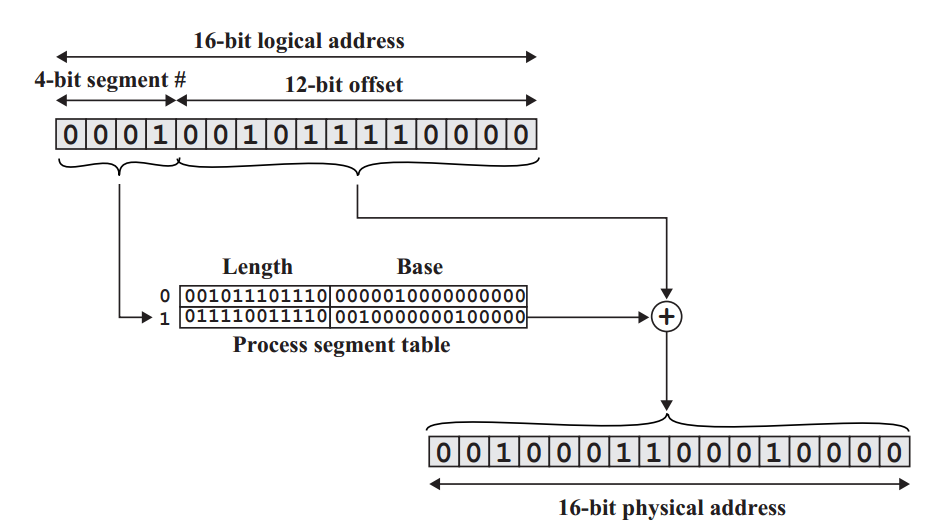
\includegraphics[scale=0.5]{segmentation}}
Primärminnet delas in i segment. En referens till en minnesplats innehåller vilket segment och en offset från segmentbasen. Får att komma åt minnet behövs oftast hela segmentet laddas in i minnet om man inte har paging. Segment är väldigt naturligt om man tänker på hur program är uppdelade i rutiner. Det delar också upp program och data. Utan segmentering skulle virtuellt minne nästan vara omöjligt. Segmentering är att föredra om man vill undvika intern segmentering och dela specifika datastrukturer mellan processer. \\ \\
Med paging innehåller segmentet flera pages och offseten omvandlas till en page som laddas in i minnet. Ett segment kan lätt expanderas genom att det får flera pages.

\subsection{MMU}
Memory management unit. Omvandlar minnesrefernser till en fysiskt adress.

\subsection{paging}
\centerline{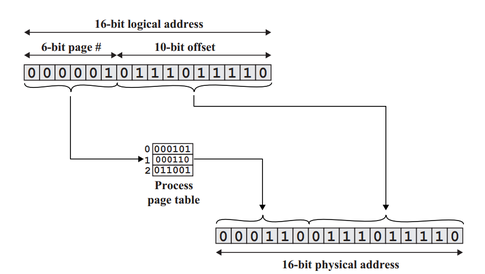
\includegraphics[scale=0.7]{paging}}
Används när man inte kan ladda hela/alla program in i ram-minnet och måste förvara en del programmet på hårddisken. Skiljer inte på program och data. Gör det enkelt att utöka minnet då det inte kräver sekventiellt fritt minne. Pages kan delas mellan processer men då är de read-only alternativt copy-on-write, dvs vill en process skriva till en sida som delas får processen en ny likadan sida.\\ \\
Om ett program försöker komma åt en sida som inte är ladded(page fault) utförs följande:
\begin{itemize}
\item hitta vart sidan ligger på hårddisken
\item hitta en tom sida i ram-minnet
\item ladda sidan till ram-minnet
\item uppdatera page-table 
\item ge tillbaka kontrol till programmet
\end{itemize}
\subsection{Thrashing}
Mycket av processertiden går åt till att ladda in sidor i ram-minnet. Kan uppkomma av att en process har får få pages att arbeta med. Kan lösas med mer ram eller minska antalet program på datorn. 
\subsection{Translation lookaside buffer}
Är ett cacheminne som omvandlar virtuella adresser till fysiska adresser. Finns den virtuella adressen in i cache så måste den söka igenom page table.

\section{virtuellt minne}
\subsection{sidtabell}
används för att omvandla den virtuella adressen till en fysiskt. Görs för varje minnesreferens så det måste gå snabbt. 
\subsection{Enhanced FIFO second-chance}
Alla sidor lagras i en ringbuffer och har en use-bit. Use-biten 1-ställs när sidan först laddas och varje gång den refereras till. Varje gång man söker igenom buffern bakifrån så 0-sätts alla use-bit. Den första med en use-bit=0 tas bort.
\subsection{Write-through}
CPU:n använder ett cache minne för att skriva till långsammare minnen. Skrivs direkt och synkront.
\subsection{delayed-write}
Datan lagras ett tag i ett temporärt minne och skrivs senare till det långsammare minnet. Bra där data används temporärt av ett program och raderas nästan direkt.

\section{Filsystem och sekundärminne}
\subsection{file control block}
Heter inode i Linux. En kopia på alla öppna fcb:s ligger i kernel minne och innehåller vad användare får göra. När den har blivit ändrad., ägare, storlek och pekare till blocken.
\subsection{soft/hard links}
mjuka länkar innehåller hela filnamnet så om namnet på en fil ändras så blir länken ogiltig. En hård länk innehåller en pekare till datan så om datan flyttas så är länken ogiltig.
\subsection{virtual file system}
ett abstraktionslager mellan os:et och hårdvaran. Detta gör det möjligt att os:et kan köras på flera olika filsystem. 
\subsection{cache}
En hårddisk har ett cacheminne som innehåller de senaste inläsningarna. Detta gör att average read time är lägre än actual read time. När os:et begär data så kan den begära mer än vad det behöver så att datan ligger i cache minnet, till exempel om det håller på att läsa in en lång fil.
\subsection{internal fragmentation}
om ett program begär 23bytes så får det 32 istället för minnet är uppdelat så.
\subsection{external fragmentation}
filer sprids på olika delar av hårddisken så det tar lång tid att läsa in hela filen.
\subsection{länkad allokering}
Varje fil är en länkad lista med diskblock. Katalogen vat första och sista pekaren. Varje block har en pekare till nästa block. 
\subsection{sammanhängande allokering}
Varje fil ligger på ett samlat ställe på disken. Katalogen vet startpekaren och storleken. 

\subsection{indexerad allokering}
Alla filer har ett indexblock som innehåller alla pekare till filens block. Katalogen vet files indexblock. Det blir ett overhead för att spara alla pekare.
\subsection{FAT}
som indexerad fast det finns en tabell över alla pekare mellan blocken. 
\subsection{inode}
Representerar en fil på en hårddisk i operativsystemet. Innehåller bland annat(POSIX):
\begin{itemize}
\item storleken på filen
\item på vilken enhet den ligger
\item användar id
\item group id
\end{itemize}
\subsection{utsvältning}
En del schemaläggningsalgoritmer kan göra så att visa processer aldrig får tillgång till CPU:n. Till exempel om man använder shortest-job first och bara tittar på hur lång tid en process tar. Då kan en process som tar lång tid bli utsvulten. För att motverka detta får man ta hänsyn till hur länge en process har väntat.
\subsection{first come first serve}
den som först begär hårddisken får först tillgång till den
\subsection{shortest seek time first}
Sökningen som ligger närmast hårddisken nuvarande position kommer först. 
\subsection{Scan algorithm}
Hårddisken åker fram och tillbaka över disken och när den är nära en sektor som nägon  vill åt hämtar den datan. 
\subsection{c-scan algorithm}
som scan fast den gör inget på tillbakavägen

\subsection{förbättre prestande}
Raid 0
\section{skydd och säkerhet}
\subsection{skydd}
mekanism som kan användas för att kontrollera tillgång till resurser.

\subsection{säkerhet}
\subsection{setuid}
Om en fil har setuid satt så körs den filen som om den vore startad av ägaren. Om en fil har setuid satt och ägs av root så kan detta vara en säkerhetsrisk. 

Skydda innehållet från yttre medveten påverkan.
\subsection{dual-mode operations}
Instruktioner som ändrar MMU-register och liknande kan inte utföras från user level programs. Endast från en interupthandler i kernel mode.
\subsection{capability list implementation}
varje användare har en lista över vad den får göra med dokument. 
\subsection{buffer-overflow attack}
När ett program medveten överskrider en buffers storlek för att skriva över data. Detta kan göra det möjligt
att attakera program och starta egna program som har samma privilegier som det attackerade programmet. Även läsa data som inte tillhör processen(heartbleed). Man kan motverka detta genom att göra boundchecks på systemanrop.
\subsection{salt hashing}
gör rainbow tables omöjliga.

 
\end{document}